\documentclass[11pt,a4paper,titlepage,spanish]{article}
\usepackage[left=1.5cm,top=2.5cm,right=1.5cm,bottom=2.5cm]{geometry} 
\usepackage[utf8]{inputenc}
\usepackage[spanish, es-tabla]{babel} %esto es para que aparezca "tabla" en lugar de "cuadro" al poner título a una tabla
\usepackage[T1]{fontenc}


%\usepackage{bbm}
\usepackage{amsthm,amsmath,mathrsfs}
\usepackage{hyperref}
\usepackage{color}
\usepackage{subfig}
\usepackage{float}

\usepackage[pdftex]{graphicx}
\DeclareGraphicsExtensions{.pdf,.png,.jpg,.bmp}

\newcommand{\HRule}{\rule{\linewidth}{0.5mm}}

% --- Para el encabezado
%\usepackage{fancyhdr}
%\fancyhead[L]{Preguntas teoricas} \fancyfoot[C]{\thepage}
%\pagestyle{fancy}
% -------------------------------------------------------- %
%opening
\title{Proyecto de grado\\ ``Análisis de video en Biomecánica''}
\author{Gonzalo Pereira. Mauricio Ramos, Guillermo Ottado, Andréi Guchin.}
\date {}

\begin{document}

\maketitle

\newpage
\tableofcontents
%\printindex
\newpage

%\begin{abstract}
%\begin{center}
%Documentación
%\end{center}
%\end{abstract}

%\clearpage


%%%%%%%%%%%%%%%%%%%%%%%%%%%%%%%%%%%%%%%%%%%%%%%%%%%%%%%%%%%%%%%%%%%%%%%%%%%%%%
%%%%%%%%%%%%%%%%%%%%%%%%%%%%%%%%%%%%%%%%%%%%%%%%%%%%%%%%%%%%%%%%%%%%%%%%%%%%%%
\chapter{Introducción}
%%%%%%%%%%%%%%%%%%%%%%%%%%%%%%%%55%%%%%%%%%%%%%%%%%%%%%%%%%%%%%%%%%%%%%%%%%%%%%%%%%%%%%%%%%%%%%%%%%%%%%%%%%%%%%%%%%%%%%%%%%%%%%%%%%
% requerimientos,Hacer como una sinopsis.
%%%%%%%%%%%%%%%%%%%%%%%%%%%%%%%%%%%%%%%%%%%%%%%%%%%%%%%%%%%%%%%%%%%%%%%%%%%%%%%%%%%%%%%%%%%%%%%%%%%%%%%%%%%%%%%%%%%%%%%%%%%%%%%%%%%

Este documento presenta las tareas realizadas en el marco del proyecto de fin de carrera ``Análisis de Video en Biomecánica'' realizado en la Facultad de Ingeniería, Universidad de la República (UdelaR). A continuación, se hace una introducción a la problemática encontrada, en función de la cual se plantea el objetivo del proyecto y una breve descripción de las soluciones actualmente disponibles.
\vspace{5 mm}

Especialistas de distintos ámbitos académicos o profesionales se encuentran habitualmente en la necesidad de realizar estudios del movimiento del cuerpo humano. Esta tarea implica registrar la posición de miembros o articulaciones en el espacio y su correspondiente evolución en el tiempo.
\\ 

Algunos ejemplos correspondientes a distintas áreas que ilustran estas necesidades son:

\begin{itemize}
\item A \emph{nivel asistencial}, en el área de \emph{fisioterapia}. Para realizar un seguimiento de la evolución de un paciente resulta importante en muchos casos conocer en detalle el movimiento, posición, etc. de la articulación o miembro afectado para llevar un control del mismo durante la rehabilitación y así poder determinar con mayor exactitud el estado y la evolución del paciente.
\item \emph{Investigación académica en biomecánica}. Diversos proyectos se llevan a cabo en las universidades sobre esta temática, por ejemplo, en la Facultad de Ingeniería de la Udelar  se realizó el estudio comparativo de la patada delfín y la patada “crawl” respecto al nado de los peces por ondulación, tratando de explicar cómo la misma puede ser propulsiva. Para ello se analizaron videos de nadadores olímpicos mediante los cuales se obtuvo una secuencia temporal de las posiciones de diferentes partes del cuerpo durante varios ciclos de patada\footnote{\textcolor{blue}{\scriptsize{\underline{\url{ http://www.fing.edu.uy/ingenieriademuestra2011/proyectos/proyectos-del-instituto-de-f\%C3\%ADsica}}}}. Accedido 20-12-14}.
\item \emph{Medidas de performance en el deporte de alto nivel}. Cuando se habla de entrenamiento deportivo se hace referencia tanto a la mejora del rendimiento del atleta como a la optimización de las capacidades en función del deporte en el que se desempeña. La técnica deportiva está relacionada directamente con la optimización de estas capacidades por lo que una buena técnica permite el mejor aprovechamiento de las posibilidades físicas del atleta garantizando mejores resultados. Las mejores soluciones para la optimización de la técnica de un deportista consisten en el análisis de videos donde se puede estudiar en detalle cada uno de los movimientos del  mismo.
\item \emph{Animación 3D}. Probablemente el más conocido de estos ejemplos, tanto en el diseño de videojuegos como en películas, programas de televisión o comerciales, muchas veces se requiere capturar el movimiento de un actor para interpretar un personaje ficticio y que sus movimientos parezcan lo más natural posible. En el medio local existen empresas que se dedican a esto, tales como Mopix \footnote{\textcolor{blue}{\underline{\url{http://mopix.com.uy/}}}. Accedido 20-12-14}.
\end{itemize}

En este contexto, el análisis de video  es  una  herramienta  fundamental para la recolección y estudio de datos. El seguimiento de puntos de referencia se utiliza para el cálculo de posición y otras variables asociadas como son la velocidad, la aceleración y por ende desplazamientos. Trabajar con video permite además estudiar secuencialmente situaciones estáticas en el tiempo. El seguimiento de dichos puntos resultaría tedioso si se hiciera manualmente por lo que resulta necesario contar con una herramienta que realice esta tarea automáticamente.
\\ 

A raíz de esto, se crean los \emph{sistemas de captura de movimiento}, que se definen como un conjunto de dispositivos y software que a partir de la grabación del movimiento de una persona (o cualquier otra cosa), es capaz de trasladar dicho movimiento a un modelo digital para diferentes fines.
\\ 

Los ejemplos mencionados anteriormente definen distintos casos de uso con características disímiles, de manera que la búsqueda de una solución única que abarque las necesidades particulares de todos ellos resulta compleja. Por ejemplo, en el ámbito deportivo la velocidad del movimiento es una variable importante a tener en cuenta para desarrollar una solución, de esta variable depende la elección tanto del sistema de adquisición como de los algoritmos más eficaces para el registro del movimiento.  De igual manera definir la portabilidad del sistema depende de si la actividad a relevar es en condiciones de laboratorio controladas o al aire libre, debido a la protección y transporte de equipos o las variaciones en las condiciones de iluminación, ruido, etc..
\\ 

Al  día  de  hoy, las  soluciones  de  software  disponibles que  podrían  asistir al especialista en su tarea, son mayormente comerciales. Las pocas alternativas de código abierto, carecen de las características necesarias para el especialista o están enfocadas hacia otras áreas de aplicación. Contar con este tipo de herramientas es fundamental para las necesidades de los equipos de profesionales, cuya alternativa son productos comerciales de alto costo.
\\ 

En virtud de estas necesidades, este proyecto busca \emph{relevar y caracterizar los distintos casos de uso para un sistema de captura de movimiento, seleccionar uno que sea representativo y suficientemente general para poder realizar una aplicación básica y funcional de código abierto de análisis de video, que proporcione solución a las necesidades que se describieron ya sea utilizando como base algún  proyecto  de  software  libre  existente, o en su defecto, desarrollando un prototipo de software básico completo que abarque el problema en forma general, para luego estudiar extender la aplicación hacia otros casos de uso}.
\\ 

Es importante resaltar la importancia de tener una primer versión del sistema de principio a fin, con todas las etapas implementadas, de forma tal de abarcar todos los procesos que la captura de movimiento implica.  Esto tiene como ventaja que se tendrá un panorama general del estado del arte de cada etapa del sistema, y 
sentará las bases para que proyectos futuros puedan optimizar individualmente dichas etapas acorde a las necesidades del cliente.
\\ 

Los requerimientos para la implementación de este sistema provienen de investigadores del Departamento de Biofísica de la facultad de medicina de la Udelar, el foco del proyecto es la investigación no asistencial pero también puede utilizarse para fines asistenciales, particularmente el estudio del movimiento de las personas.
\\ 

De acuerdo a lo planteado por el cliente y a las hipótesis que se establecieron en conjunto, se plantean los siguientes supuestos relativos a la apariencia del laboratorio:
\begin{itemize}
\item Las capturas de movimiento del paciente se realizan en un ambiente controlado:\vspace{-0.2cm}
	\begin{itemize}
		 \item La iluminación es la adecuada para realizar las  capturas correctamente.
		 \item El fondo sobre el que se hacen las capturas es estático, de color oscuro y opaco.		 
		 \item Se utiliza cámaras convencionales y la ubicación de las cámaras así como sus parámetros de interés son conocidos.
	\end{itemize}
	\vspace{-0.2cm}
\item La vestimenta que utiliza el paciente es oscura, opaca y lo más ajustada al cuerpo como sea posible.\vspace{-0.1cm}
\item Los marcadores a detectar son esferas blancas colocadas convenientemente sobre el cuerpo del paciente.
\end{itemize}

En cuanto al movimiento se asume que:
\begin{itemize}
\item El paciente permanece dentro del área de captura.\vspace{-0.1cm}
\item Existe oclusión de marcadores en vistas dadas.\vspace{-0.1cm}
\item Las cámaras se mantienen fijas.
\end{itemize}

Por otro lado, como se muestra en la Figura \ref{abuela2} se requiere que la salida del sistema sea la posición en el espacio 3D de los marcadores, ubicados en el cuerpo del paciente, en cada instante de la captura, con la correcta identificación de dichos marcadores en cada cuadro. A estos requerimientos, se le suman otros de carácter académico, como la importancia de tener una base de datos con un cierto número de secuencias y una método de evaluación de performance establecido. Estos dos aspectos toman gran relevancia en etapas futuras, de ampliación de este proyecto, ya que al realizar pruebas  de nuevas implementaciones sobre los mismos datos y evaluar los resultados con iguales métricas se tiene un punto de referencia sobre el cual evaluar posibles mejoras del sistema.
\\ 

En resumen, el sistema creado pretende bajo ciertas condiciones controladas, obtener las coordenadas espaciales de un número de puntos de interés sobre una paciente. Una de las formas de obtener esto, y la estudiada en este trabajo, es colocar al sujeto con traje negro con marcadores en un ambiente con iluminación adecuada, filmar con varias cámaras a lo largo del tiempo, adquirir esta información en la computadora y mediante un posterior procesamiento obtener la posición 3D de cada uno de los puntos de interés (los marcadores) a lo largo de toda la secuencia.

\begin{figure}[H]
\begin{center}
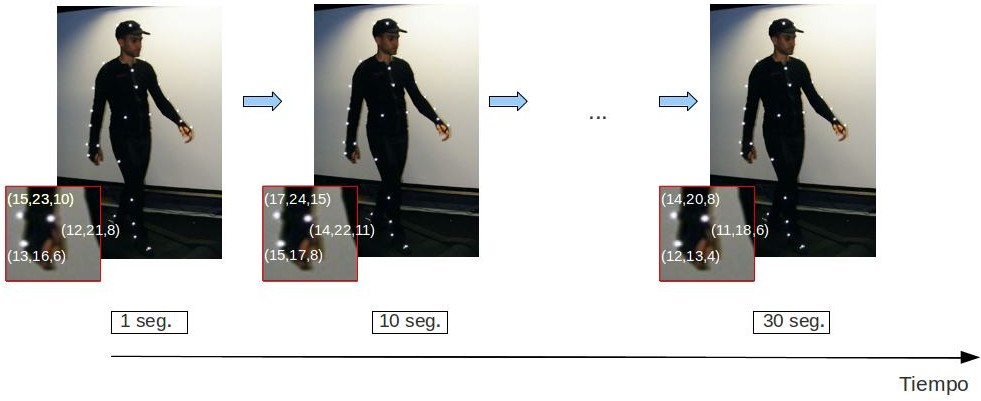
\includegraphics[scale=0.4]{img/Sistema_completo/diagrama_abuelas_2.jpg}
\end{center}
\caption{Posición de los marcadores a lo largo del tiempo.}
\label{abuela2}
\end{figure}

La aplicación recibe como entrada imágenes de video provenientes de varias cámaras, las cuales capturan el movimiento de una persona desde distintos ángulos. Se implementan métodos que permiten obtener información sobre las cámaras y su disposición en el espacio mediante la calibración. Con esta información y a partir de las imágenes obtenidas se detectan distintos puntos de referencia del cuerpo según el estudio particular que se desee realizar. Posteriormente, a partir de la información de las múltiples cámaras se reconstruye la posición 3D de los puntos en cada cuadro, para luego efectuar la identificación de trayectorias de los puntos de interés a lo largo de la secuencia, ver Figura \ref{abuela1}. A partir del procesamiento de la posición 3D de los puntos se obtendrán otros datos estadísticos de interés para el usuario.\\

\begin{figure}[ht!]
\begin{center}
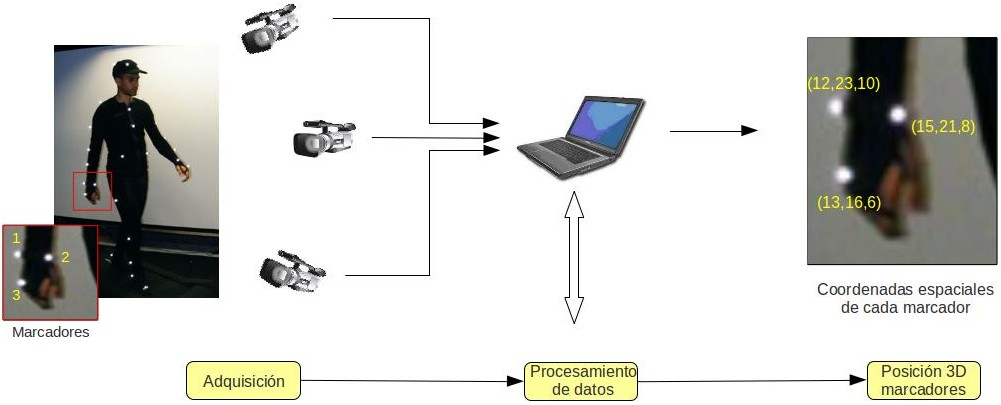
\includegraphics[scale=0.4]{img/Sistema_completo/diagrama_abuelas_1.jpg}
\end{center}
\caption{Funcionamiento de un sistema de captura de movimiento.}
\label{abuela1}
\end{figure}


%SINOPSIS
El proyecto se inicia con investigación y revisión bibliográfica sobre la temática, buscando diseños provenientes de sistemas de captura de movimiento ya implementados, así como  detalles sobre la implementación parcial o total de cada funcionalidad de interés. 
\\ 

Rápidamente se procuró obtener una base de datos con secuencias, ya sean reales o sintéticas, sobre los cuales implementar la aplicación y sus distintos bloques. Si bien esta búsqueda no aportó los resultados esperados,
%no obtuvo buenos resultados %ME QUERES MATAR ANDREI!!!!
 debido a que no se encontraron bases de datos acorde a las necesidades del proyecto, se implementa un prototipo de base de datos sintética con un número reducido de secuencias como alternativa tomando algunos conceptos encontrados en dicho relevamiento, generando una base flexible, de fácil expansión y con potencial para futuros estudios.\\ 

 Luego de analizar la bibliografía y definir la metodología, se opta por implementar el sistema con los 4 bloques principales mostrados en la Figura \ref{bloquesSistintro}. 

 \begin{figure}[H]
\begin{center}
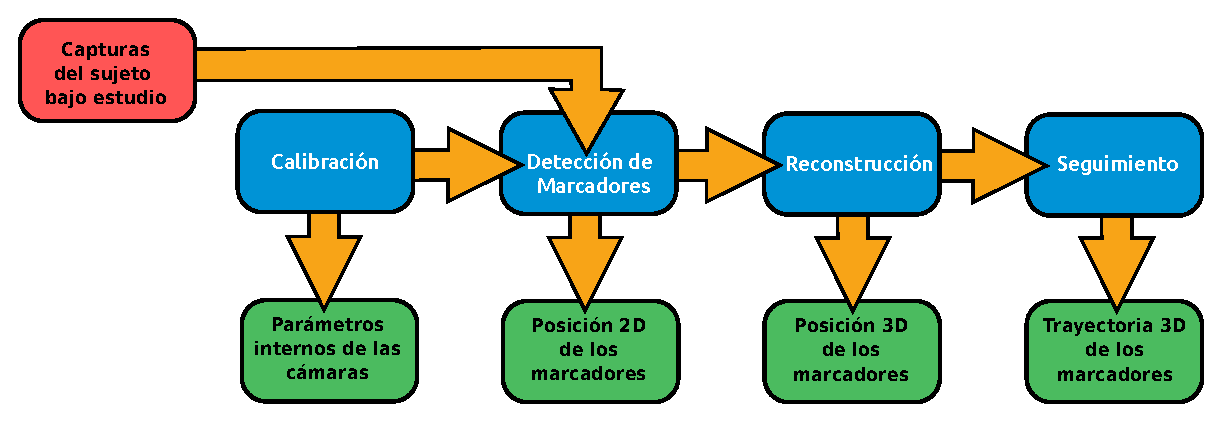
\includegraphics[scale=0.7]{img/Sistema_completo/Diagrama_de_bloques.eps}
\end{center}
\caption{Diagrama de bloques del sistema a implementar.}
\label{bloquesSistintro}
\end{figure}

Cada uno de estos bloques cumple un objetivo definido:
\begin{itemize}
\item El bloque de \emph{calibración}, es el encargado de obtener los parámetros internos y externos de las múltiples cámaras utilizadas en la captura, permitiendo establecer la relación entre el espacio ambiente y la imagen sobre cada cámara. Una vez que se disponen el número y posición de las cámaras para efectuar la captura de movimiento, este bloque releva por única vez la información previa necesaria para realizar una correcta reconstrucción de los puntos.
\item El bloque \emph{detección de marcadores}, identifica los marcadores en las imágenes obteniendo la posición 2D de cada uno de ellos a lo largo de la secuencia de captura en cada cámara (ver Figura \ref{peladocirculosintrointro}).
\item Con información de posición 2D proveniente de la detección de marcadores en múltiples vistas, y los parámetros relevados en calibración, el bloque de \emph{reconstrucción} (ver Figura \ref{peladoewconstruidointro}) se encarga de obtener la posición 3D de cada marcador.
\item Por último, el bloque de \emph{seguimiento} (ver Figura \ref{peladoetrackingintro})
(o ``tracking'') relaciona cada marcador en determinado cuadro de la secuencia con los que le siguen en el resto de los cuadros, obteniendo así la trayectoria de cada marcador a lo largo del tiempo.
\end{itemize}

Cabe destacar que estos bloques se implementaron de manera independiente, con una interfaz claramente definida, de manera  de poder realizar modificaciones sobre uno de ellos sin afectar el funcionamiento de los otros. Este aspecto cobra relevancia en etapas futuras, donde bajo la necesidad de optimizar algún bloque en particular o agregar alguna nueva característica que permita procesar datos provenientes de nuevos casos de uso, se deba modificar el sistema. De no presentar esta particularidad, la modificación de un bloque podría afectar negativamente el funcionamiento del sistema completo, requiriendo una posible re-ingeniería de la estructura.

\begin{figure}[ht!]
        \centering
        \hspace{1.3 cm}
        \subfloat[Captura original]{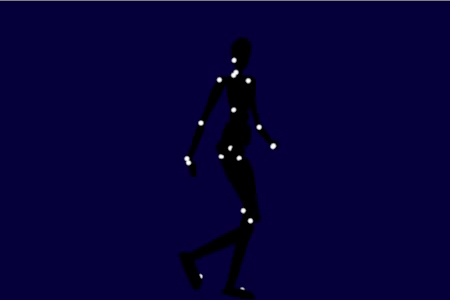
\includegraphics[scale=0.4]{img/peladoFondoAzul.png} %\label{peladoOriginalintrointro}
        }\hspace{2.2 cm}
        \subfloat[Detección de marcadores]{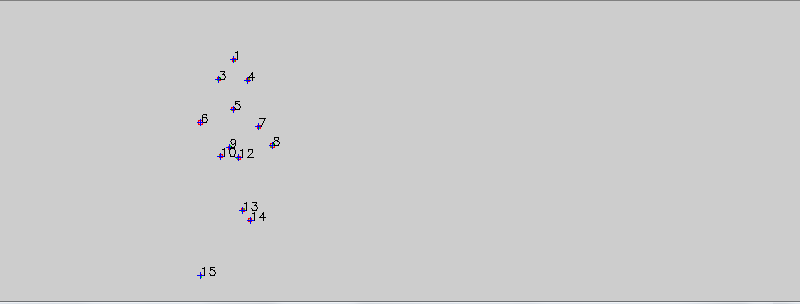
\includegraphics[scale=0.4]{img/peladoFondoAzul_circulos.png}\label{peladocirculosintrointro}}

        \subfloat[Recontrucción 3D]{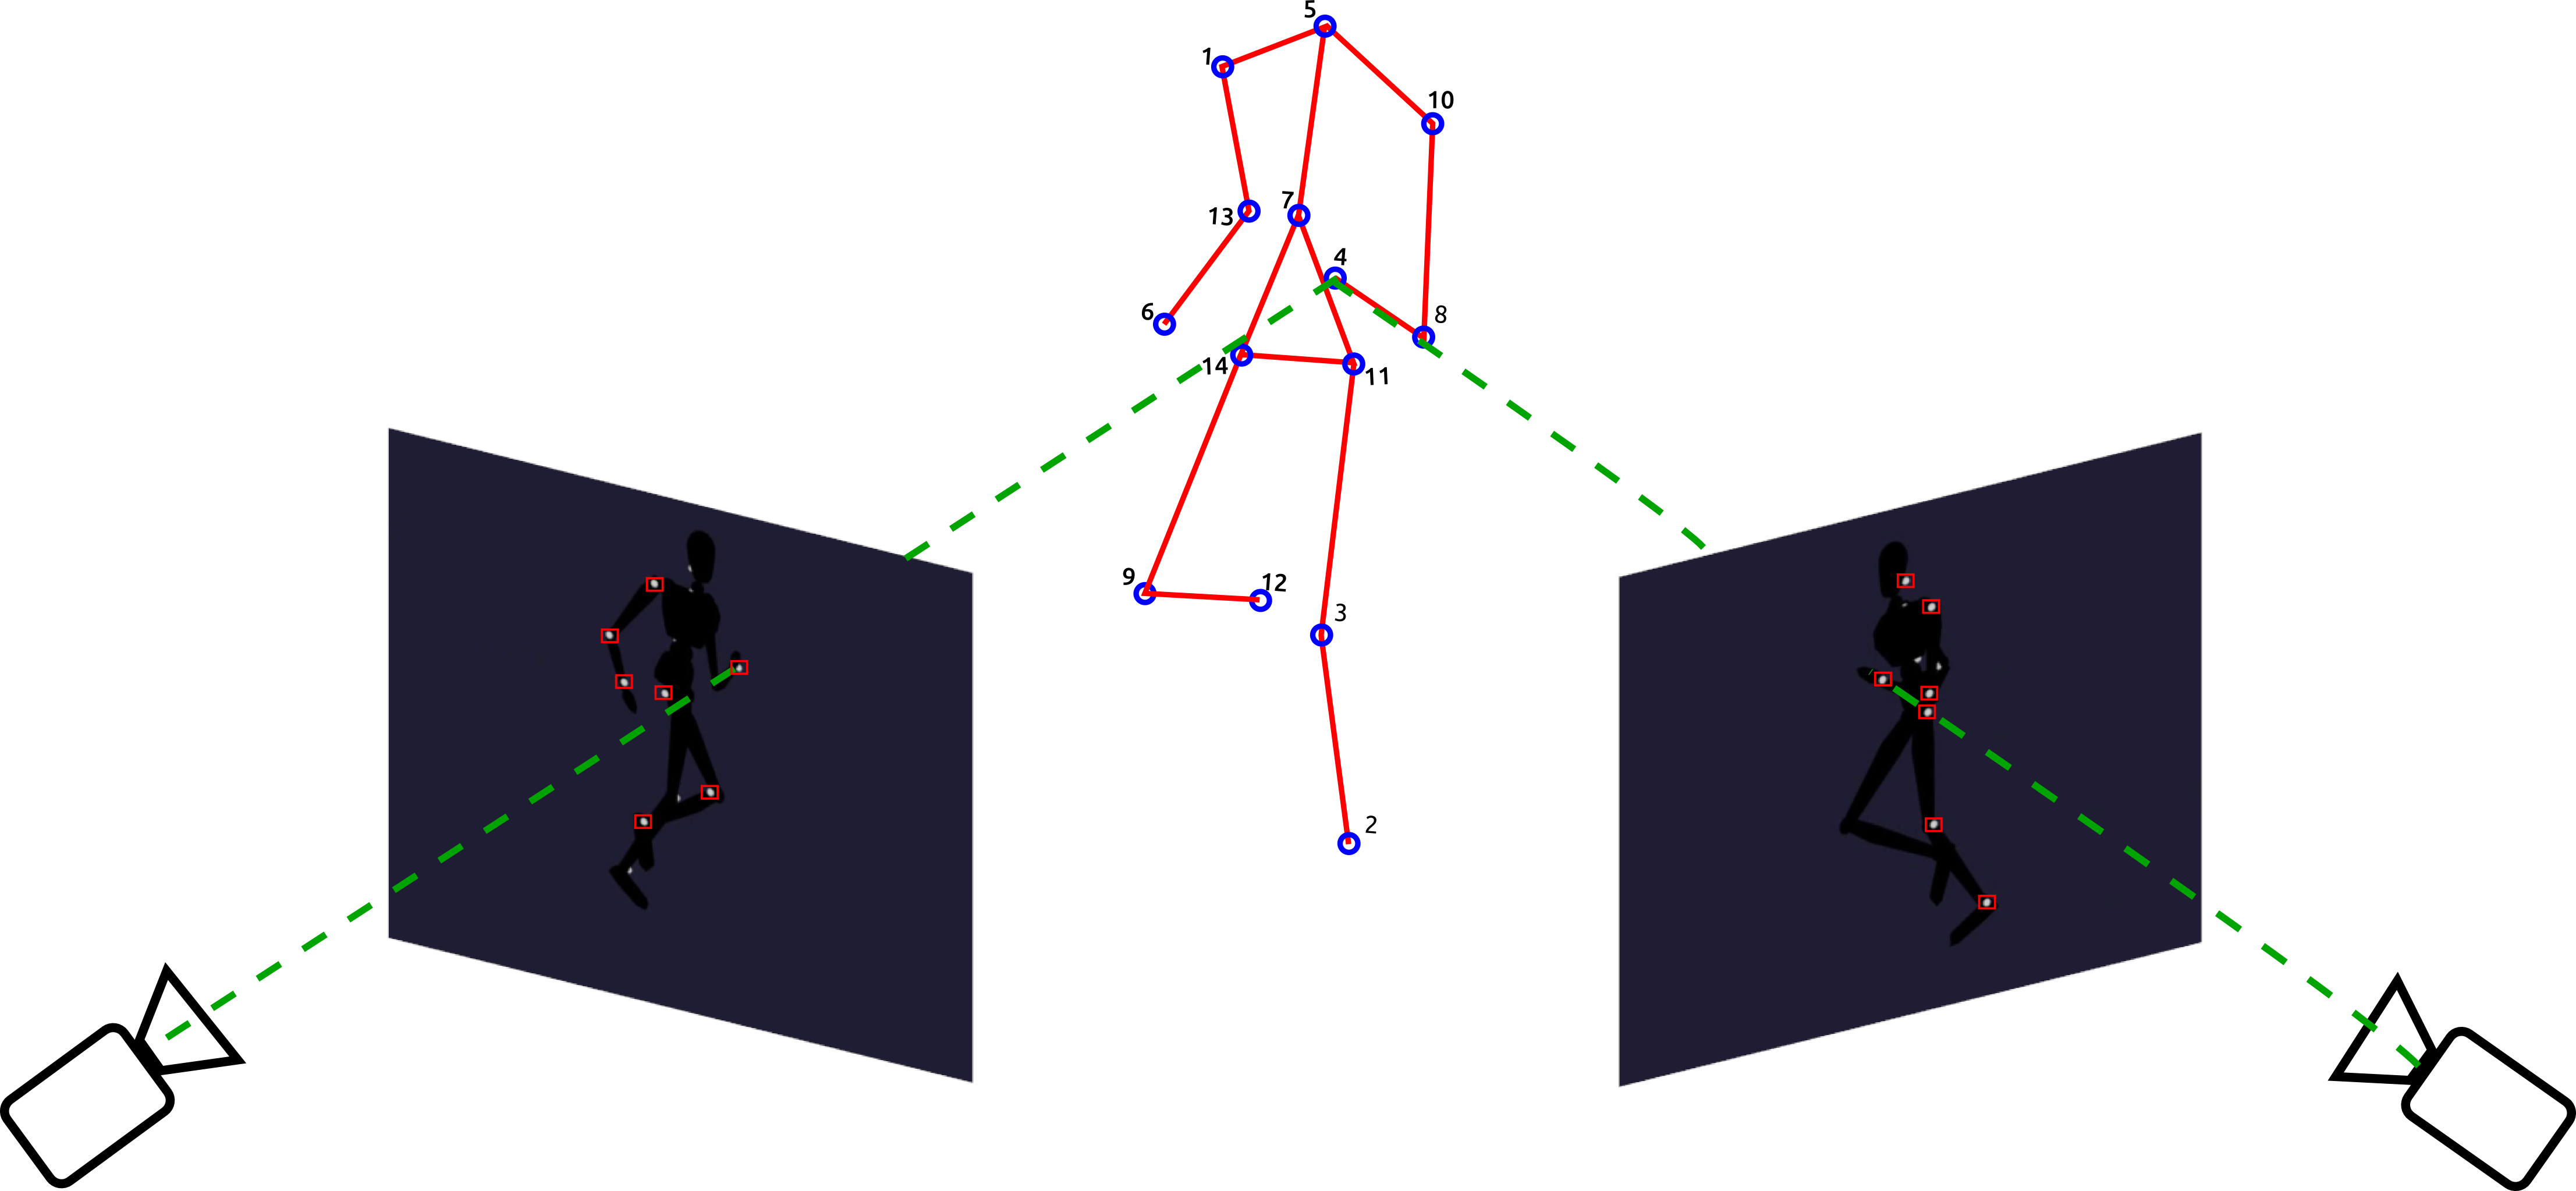
\includegraphics[scale=0.15]{img/Reconstruccion/reconstruccion1.png}\label{peladoewconstruidointro}}
    	\subfloat[Seguimiento]{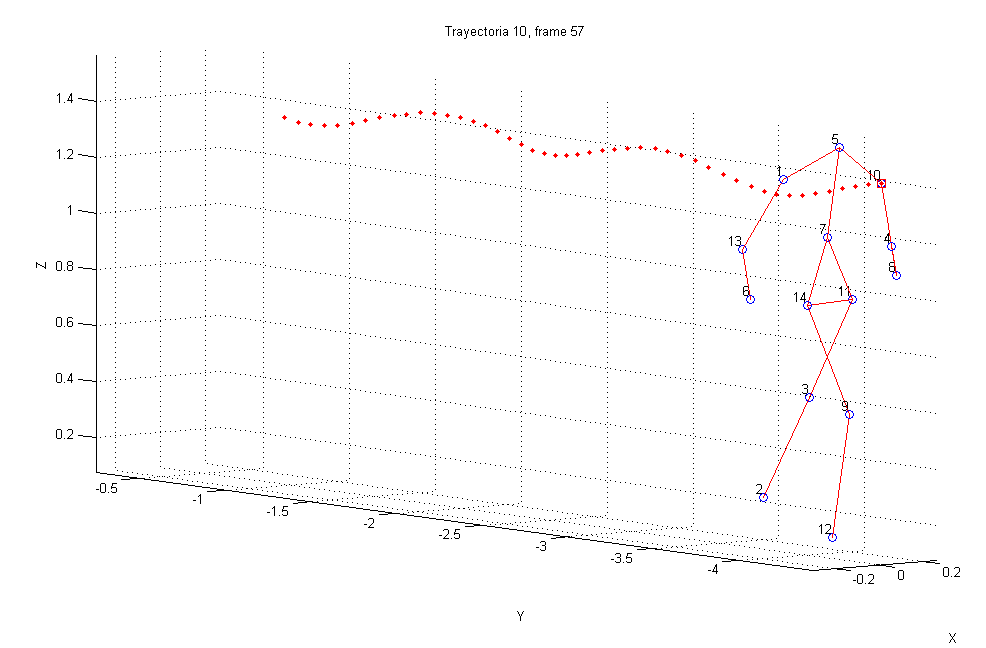
\includegraphics[scale=0.24]{img/Tracking/track1.png}\label{peladoetrackingintro}}  
  \caption{Salidas de los bloques principales del sistema.}
      \label{ejemplotutiintro}
\end{figure}

Por otro lado, fue elaborada una interfaz gráfica básica de forma tal de facilitar la ejecución del software para los usuarios sin tener que trabajar directamente con el código.
\\ 

A continuación se presenta una breve revisión del estado del arte de los sistemas de captura de movimiento disponibles. Una descripción más detallada y más técnica se realizará en la Sección \ref{invBiblio}, luego se define el objetivo del proyecto y se comenta la estructura de la documentación.

\section{Estado del arte}
%%%%%%%%%%%%%%%%%%%%%%%%%%%%%%%%%%%%%%%%%%%%%%%%%%%%%%%%%%%%%%%%%%%%%%%%%%%%%%%%%%%%%%%%%%%%%%%%%%%%%%%%%%%%%%%%%%%%%%%%%%%%%%%%%%%5
%qué opciones tengo para hacerlo? por qué hay estas opciones? para qué se usan?
%%%%%%%%%%%%%%%%%%%%%%%%%%%%%%%%%%%%%%%%%%%%%%%%%%%%%%%%%%%%%%%%%%%%%%%%%%%%%%%%%%%%%%%%%%%%%%%%%%%%%%%%%%%%%%%%%%%%%%%%%%%%%%%%%%%

Al día de hoy existen varios sistemas de captura de movimiento, sin embargo los mas usados debido a su buena performance y soporte presentan altos costos de licenciamiento. 
\\ 

Como se mencionó anteriormente, los más populares en la actualidad son los que se utilizan en la industria del cine o del diseño de videojuegos. En este contexto, se almacenan las acciones de actores humanos y se usa esta información para animar modelos digitales de personajes en animación 3D.
\\ 

Algunos ejemplos de sistemas de captura de movimiento bajo licencia son:

\begin{itemize}
\item \emph{Vicon} \cite{vicon}. Es una empresa que vende sistemas de captura de movimiento, tanto software como hardware. Sus sistemas son muy conocidos y fuertemente utilizados en estudios clínicos y biomecánicos alrededor del mundo, así como para otras investigaciones científicas. En particular, este sistema está siendo utilizado en el Departamento de Fisiatría y Rehabilitación del Hospital de Clínicas. Presenta como ventajas frente a otros sistemas la velocidad con que realiza el procesamiento de los datos y la calidad de las cámaras para realizar las capturas. La gran desventaja que posee es el alto costo de sus equipamientos, bastante privativo en algunos ámbitos.
\item \emph{Qualisys} \cite{qualisys}. Junto con Vicon son los dos sistemas de captura de movimiento más utilizados en el ámbito de la investigación científica. Presenta como ventajas frente al anterior la utilización del modelo AIM\footnote{Automatic Identification of Markers}, un identificador de marcadores que ``aprende'' de cada secuencia procesada ahorrando mucho tiempo y trabajo en identificar marcadores. Además presenta una interfaz de usuario más amigable y requiere menos tiempo de capacitación para su uso.
\item \emph{OptiTrack} \cite{optitrack}. Es de los sistemas comerciales de menor costo, cerca de la cuarta parte de lo que cuesta un sistema Vicon. Otra de sus ventajas es que brinda acceso de bajo nivel a través de un conjunto de  SDK's y API's tanto para el hardware como para los datos obtenidos, permitiendo manipular los mismos y procesarlos de la manera deseada por fuera de las aplicaciones que originalmente provee. 
\item \emph{Massive} \cite{massive}. Es un software destinado a producir efectos especiales para cinematografía, programas televisivos y videojuegos entre otras cosas. El software implementa la captura de movimiento y cuenta con varios productos para generar distintos tipos de efectos y animaciones. Fue originalmente diseñado par utilizar en la trilogía de El Señor De Los Anillos de Peter Jackson y desde entonces se ha convertido en uno de los mejores software para realizar efectos visuales de muchedumbres y animación de personajes autónomos.
\item \emph{Motion Analysis} \cite{motion_analysis}. es el mayor fabricante mundial de sistemas de instrumentación óptica de alto rendimiento que permite testear y medir el movimiento de los objetos. Mantiene y comercializa el software con sus sistemas de hardware. Sus sistemas evalúan el movimiento en distintas aplicaciones: producción de animación, análisis de movimiento, y en el ámbito industrial. Posee un gran número de aplicaciones de pos-producción.

\item \emph{PhaseSpace} \cite{phasespace}. Posee un sistema de captura patentado basado en marcadores leds, de alta resolución temporal y espacial. Todo el sistema se compone de sólo unos pocos elementos robustos y portátiles. Sus aplicaciones funcionan tanto en entornos Linux como Windows. Ha desarrollado soluciones de captura de movimiento para la investigación, la industria y las comunidades de las artes gráficas, también para estar al alcance de las pequeñas empresas, universidades y particulares.
\end{itemize}

Los sistemas anteriores, y la mayoría de los sistemas modernos que efectúan capturas de movimiento, utilizan sensores infrarrojos o LEDs para efectuar el seguimiento de puntos. Los segundos facilitan la etapa de detección de marcadores en cada cámara, mientras que los primeros no tienen una etapa de detección en cada vista ni reconstrucción ya que los mismos ofrecen la información de posición directamente.
\\ 

La gran desventaja de los sistemas anteriores es su alto costo. A modo de ejemplo, un sistema Vicon de 10 cámaras tiene un valor que ronda los U\$S\;70.000 \footnote{Este precio depende fuertemente del tipo de cámara que se utilice, los precios de las mismas se encuentran a partir de los U\$S\;3.000 por unidad.}.
\\ 


Por otro lado, también existen programas de captura de movimiento de código libre, un ejemplo de ello es el programa Kinovea \cite{kinovea}. Enfocado principalmente en el ámbito deportivo, permite analizar y mejorar la técnica de los atletas a través del procesamiento de secuencias de video. Posee algunas características interesantes como la posibilidad de efectuar medición de distancias, ángulos y tiempos manualmente, así como la utilización de seguimiento semi-automático de puntos en tiempo real para obtener su trayectoria. La gran desventaja que presenta frente a otros sistemas es que efectúa únicamente análisis sobre dos dimensiones y con una sola cámara.\\

Otra alternativa sobre la que se investigó es DVIDEOW \cite{figueroa2003flexible}. Este software presenta varios conceptos teóricos como primer acercamiento al problema, pero la implementación presenta pérdidas de marcadores que requieren correcciones constantes. Además, no se tiene una actualización del mismo desde el 2009, desde esa fecha a la actualidad solamente se encontraron trabajos que lo presentan como fundamento teórico.

\section{Estructura de la documentación}

Este proyecto estudia el problema de captura de movimiento y sus distintas componentes, para desarrollar un conjunto de datos y presentar un análisis sobre los mismos. 
\\

En este capitulo se presentó el objetivo general del proyecto y un breve estado del arte de la temática que será desarrollado profundamente en el Capítulo~\ref{invBiblio}, junto a un planteo en la Figura~\ref{bloquesSistintro} de los bloques que se estudiarán a lo largo del proyecto. 
\\

El Capítulo~\ref{section_base_de_datos} presentará un estudio de bases de datos disponibles y como fueron generadas capturas experimentales propias sobre las cuales trabajar. Luego el Capítulo~\ref{sec:implementacion_bloques_sistema} presentará detalles sobre el procedimiento de la Figura~\ref{bloquesSistintro} a partir de los datos experimentales generados. 
\\

En los capítulos siguientes se presentará como fue estudiado e implementado cada bloque: Segmentación y Filtrado en el Capítulo~\ref{deteccionMarcadoresSec} para la detección de la posición de los marcadores en cada video, Calibración en el Capítulo~\ref{calibracion} donde se mostrará como se genera la información del espacio de captura necesaria para luego en el Capítulo~\ref{reconstruccion} sobre Reconstrucción, mostrar como se combina la información de los bloques anteriores para calcular la posición en el espacio de los marcadores. 
\\

Posteriormente, el Capítulo~\ref{seguimiento} sobre Seguimiento propone un método de identificación de marcadores reconstruidos. 
\\

Finalmente se presenta como fue evaluado cada bloque y múltiples pruebas sobre el sistema completo en el Capítulo~\ref{evaluacion} para luego presentar las conclusiones en el Capítulo~\ref{conclusiones}.


 
  


%Dada las características de este proyecto otro antecedente relevante a tener en cuenta en el área, es el de un grupo de investigadores del Hospital de Clínicas que junto al grupo de Tratamiento de Imágenes de la Facultad de Ingeniería han estudiado previamente la marcha de las personas a los efectos de reconocer en ellas patrones de movimiento. Dicho proyecto recibe el nombre “Cíclope”.

\chapter{Implementación de bloques del sistema}
\label{sec:implementacion_bloques_sistema}

%COMENTARIO: ACÁ SE ME OCURRE DE HACER UNA INTRODUCCIÓN A CADA BLOQUE DEL SISTEMA, JUSTIFICAR Y EXPLICAR MEDIO POR ARRIBA Y EN LAS SIGUIENTES SECCIONES EXPLICAR LOS DETALLES MÁS TÉCNICOS DE CADA BLOQUE.

En base a lo estudiado en la etapa de investigación, se pudo concluir que un sistema de captura de movimiento con las características necesarias para cumplir el objetivo del proyecto debe estar formado por 4 bloques generales: \emph{calibración}, \emph{detección de marcadores}, \emph{reconstrucción} y \emph{seguimiento}. En la figura \ref{bloquesSist} se muestra un esquema del sistema a implementar.

\begin{figure}[H]
\hspace{-0.5cm}
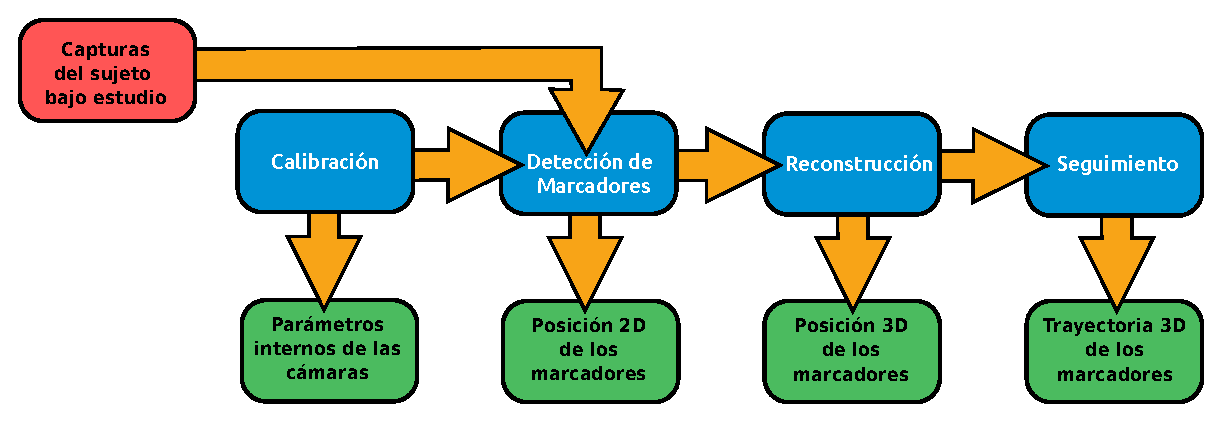
\includegraphics[scale=0.7]{img/Sistema_completo/Diagrama_de_bloques.eps}
\caption{Diagrama de bloques del sistema completo.}
\label{bloquesSist}
\end{figure}

A grandes rasgos, el sistema funciona de la siguiente manera:

\begin{enumerate}
	\item Se \emph{calibran} las cámaras. Esto es, determinar los parámetros de las mismas de forma tal de tener un mapeo del espacio 3D a las coordenadas 2D de las imágenes capturadas.
	\item Se realiza la captura del paciente en movimiento desde todas las cámaras calibradas.
	\item A partir de las secuencias, se realiza la \emph{detección de marcadores} para cada cámara. Esto equivale a determinar la posición 2D de dichos marcadores en cada cámara donde están visibles, a lo largo de toda la secuencia.
	\item Luego, con la posición 2D de determinado marcador en al menos 2 cámaras se realiza la \emph{reconstrucción} del mismo, es decir, obtener las coordenadas 3D de dicho marcador. Se realiza para todos los marcadores, y para todos los cuadros de la secuencia.
	\item Finalmente, se realiza el \emph{seguimiento} (o \emph{tracking}) de cada marcador en el espacio. Con esto se obtienen las trayectorias 3D de todos los marcadores en el cuerpo del paciente.
\end{enumerate}

Debido a los tiempos disponibles para realizar el proyecto en su totalidad, y junto a la planificación realizada al comienzo del mismo, se tiene como idea principal el conseguir la implementación de un sistema con características similares, adaptando el mismo para cumplir los objetivos establecidos. 

Sin embargo en la investigación bibliográfica se encuentra otra realidad, puesto que no hay muchos sistemas a disposición. Por un lado, la mayor parte de los sistemas encontrados poseen altos costos de licenciamiento (por ejemplo Vicon\footnote{http://www.vicon.com/, Noviembre 2014}, OptiTrack\footnote{http://www.naturalpoint.com/optitrack/, Noviembre 2014}, PhaseSpace\footnote{http://www.phasespace.com/index.html, Noviembre 2014}, Qualisys\footnote{http://www.qualisys.com/, Noviembre 2014} o MotionAnalysis\footnote{http://www.motionanalysis.com/index.html, Noviembre 2014}) y por otro lado, los sistemas de código abierto no se adaptaban a las necesidades presentes o el trabajo a realizar sobre los mismos era más Costoso que hacer una implementación propia. En este último caso se encuentra el software Kinovea\footnote{http://www.kinovea.org/, Noviembre 2014}, que realiza únicamente el seguimiento en coordenadas 2D.

Debido a los inconvenientes planteados, se decide realizar una implementación propia de los bloques del sistema. Nuevamente, de acuerdo a la filosofía explicada en los párrafos anteriores, se prioriza la búsqueda de sistemas ya implementados cuyo diseño se corresponda a cada bloque de la Figura \ref{bloquesSist},  antes de recurrir a la creación de uno.

Se tuvo presente en esta búsqueda el hecho de poder separar el sistema en bloques independientes. Esto asegura que la construcción de uno de ellos no dependa del correcto funcionamiento de otro. Por otro lado, da la posibilidad que en etapas futuras se pueda realizar el estudio de uno de los bloques de la Figura \ref{bloquesSist} individualmente y así poder modificarlo u optimizarlo sin afectar al resto. Esta forma de trabajo funciona adecuadamente siempre y cuando la salida de un bloque sea exactamente la entrada del siguiente, para los casos en que no se logra esto, se realizan algoritmos capaces de importar la salida de un bloque y convertirla al formato de entrada de otro (por ejemplo, \textit{Xml2Struct} que convierte el xml que tiene como salida el bloque de detección de marcadores en estructuras de Matlab para realizar la reconstrucción).

Como se menciona anteriormente, en la búsqueda realizada se encuentra la tesis de doctorado de Lorna Herda\cite{herda}, la misma plantea un sistema de captura de movimiento con las características buscadas para este proyecto. Al estudiar dicho sistema se encuentra que posee las mismas hipótesis de uso que el estudio preliminar realizado (utilización en fisioterapia, biomecánica, animación, deporte, etc.). Además, es un trabajo mencionado repetidas veces en otros artículos de la misma rama científica, encontrándose una documentación amplia respecto a la metodología implementada.

Debido a las ventajas que presenta esta metodología respecto a las otras encontradas, se decide implementar el sistema de Herda y elaborar los bloques de calibración y detección de marcadores aparte.

Estudiado el diseño propuesto por Herda para su sistema, se construye un diagrama de bloques completo, más detallado que el mostrado en la Figura \ref{bloquesSist}, el cual se puede observar en la Figura \ref{diagBloq}. Es importante destacar que, si bien la mayor parte de los bloques de reconstrucción y seguimiento se realizaron con la metodología del sistema de Lorna Herda\cite{herda}, en la documentación se presentan ciertas ambigüedades respecto a la descripción de algunos métodos y en la forma de resolver determinados casos de uso, que tuvieron que ser analizados y definidos por el grupo del proyecto en base a los conocimientos adquiridos.

A continuación se muestra el diagrama de bloques y se explica su funcionamiento.

\section{Diagrama de bloques}

\vspace{-0.5cm}
\begin{figure}[ht!]
\hspace{-1cm}
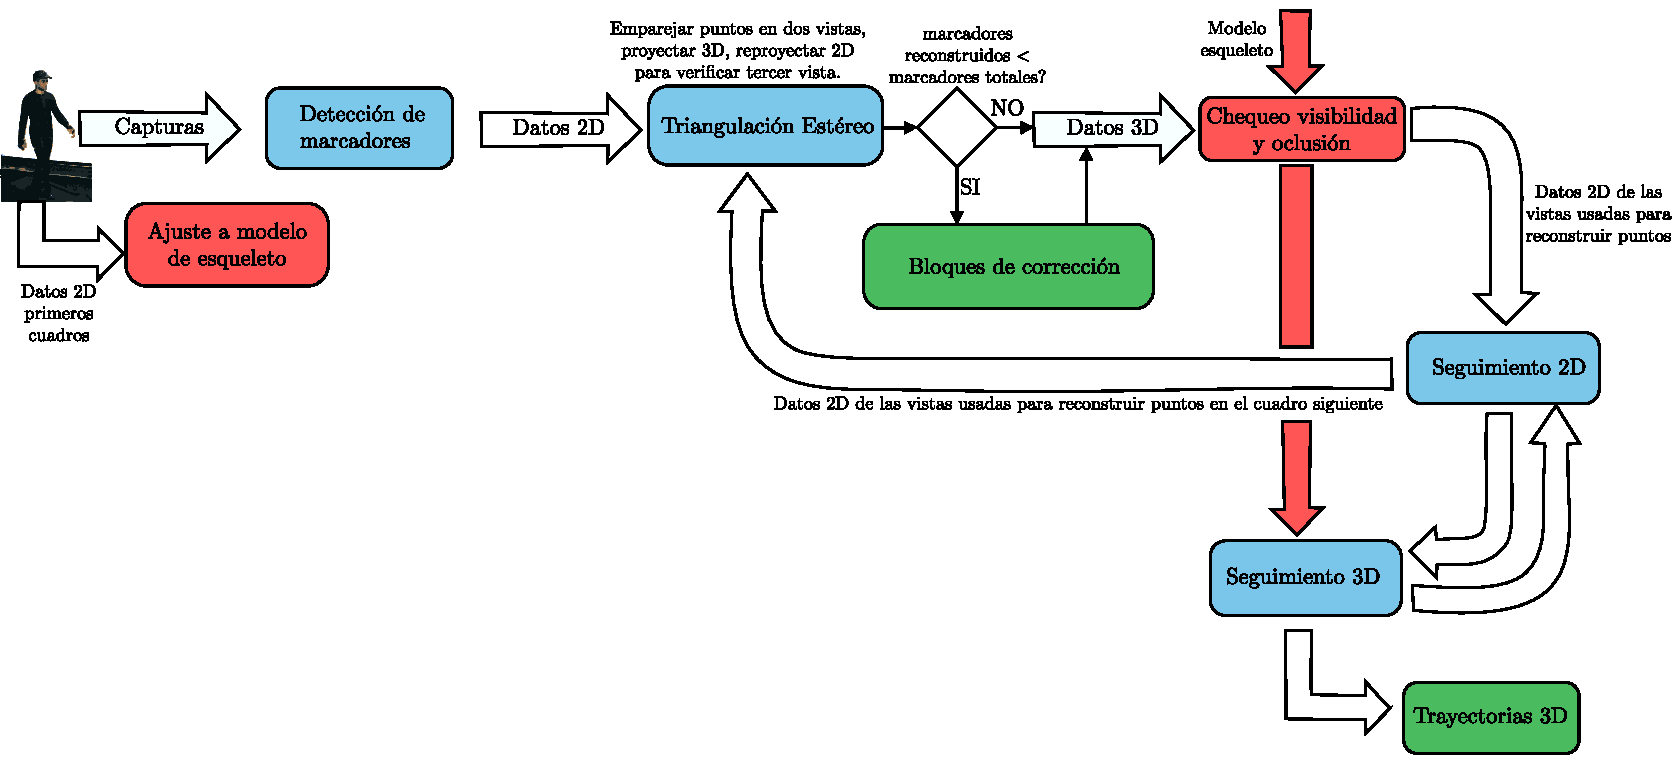
\includegraphics[scale=0.55]{img/Sistema_completo/Diagramadebloques_Herda.pdf}
\vspace{-1cm}
\caption{Diagrama de bloques detallado del sistema.}
\label{diagBloq}
\end{figure}

El sistema representado en este diagrama, funciona de la siguiente manera:

\begin{enumerate}
\item Se realiza la captura de movimiento del paciente desde múltiples vistas, en un entorno controlado. Estas capturas son la entrada principal al sistema.
\item A partir de las capturas, por un lado se ajusta el \textbf{modelo teórico de esqueleto} a utilizar, de acuerdo a las características del cuerpo del paciente, y por otro lado se realiza la \textbf{detección de marcadores} de cada cuadro para cada cámara. Este bloque es el mismo que el del diagrama de la figura \ref{bloquesSist} y se explicará en detalle en el Capítulo \ref{deteccionMarcadoresSec}.
\item Luego que se tiene la posición 2D de los marcadores en cada cuadro y en cada cámara, se realiza la \textbf{triangulación estéreo} para obtener la posición 3D de los mismos. A grandes rasgos, la \emph{triangulación 3D} empareja dos puntos en correspondencia de dos vistas distintas y con ellos calcula la proyección 3D de ese punto en el espacio, luego se re-proyecta ese punto en las otras vistas para verificar. Si verifica su posición en al menos una vista más, entonces la posición 3D se considera válida.
\item Si el número de marcadores reconstruidos en 3D es menor al número total de marcadores en el modelo de captura, se ingresa en el \textbf{bloque de corrección}, donde se utilizan varios métodos para recuperar la posición 3D de los marcadores restantes (ver Figura \ref{fig:bloqCorr}). 
\item Cuando se tiene la posición 3D de todos los marcadores, se ingresa en el bloque de \textbf{chequeo de visibilidad y oclusión} donde se verifica que la posición reconstruida de cada marcador sea correcta y no se haya reconstruido alguno con datos erróneos.
\item Finalmente, se realiza el \textbf{tracking 3D y 2D} en simultáneo para reconstruir las trayectorias de cada marcador.
\end{enumerate}

La explicación detallada de cada bloque y cómo fueron implementados se muestra en los capítulos siguientes.

A continuación, se explica como funciona el bloque de corrección:

\begin{figure}[H]
\hspace{-1cm}
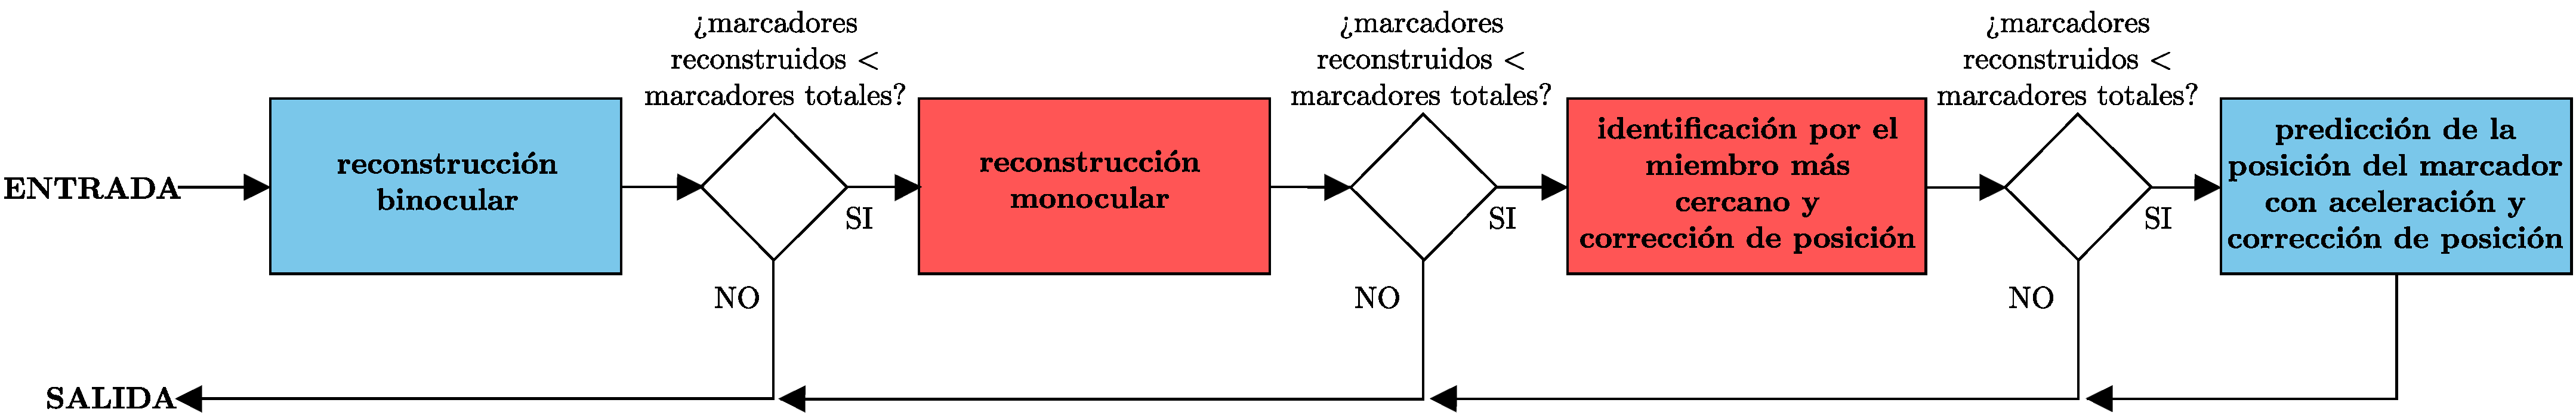
\includegraphics[scale=0.22]{img/Sistema_completo/BloquesDeCorreccion}
\caption{Detalle del bloque de corrección.}
\label{fig:bloqCorr}
\end{figure}

Una vez realizada la triangulación estéreo, se verifica que el número de marcadores reconstruidos sea igual a la cantidad de marcadores que efectivamente se estén usando en la adquisición de datos. Si esta condición no se verifica, se ejecuta un “bloque de corrección” para solucionarlo. Dicho bloque a su vez, contiene  varios sub-bloques, los cuales pueden verse en la figura \ref{fig:bloqCorr}.

Primeramente se efectúa la \emph{reconstrucción binocular} y si aún no se obtienen todos los marcadores se efectúa la \emph{reconstrucción monocular}, se disminuye la exigencia sobre la reconstrucción al utilizar sucesivamente métodos menos precisos, con el fin de completar el número de \emph{marcadores reconstruidos}.

 Si en la salida de cada uno de los bloques anteriores la condición de \emph{todos los marcadores reconstruidos} aún no se cumple, se pasa al siguiente bloque, donde se asocian los marcadores 3D reconstruidos que aún no fueron identificados con aquellas articulaciones del modelo de esqueleto (ajustado en la inicialización) que no tienen ningún marcador asociado. Para esto, se evalúan las distancias de los marcadores no identificados con la posición de las articulaciones del modelo en cuadros anteriores y se asocian aquellos marcadores que se encuentren a menor distancia a cada una de dichas articulaciones. Al tiempo que se realiza esto, se verifica que la distancia entre marcadores asociados a un mismo hueso del esqueleto se mantenga aproximadamente constante (dado que los marcadores están fijos en los huesos y los mismos no varían su tamaño).
 
Si aún faltan marcadores sin reconstruirse, se utiliza como último recurso la estimación de la posición del marcador evaluando la aceleración del mismo en cuadros anteriores y verificando que dicha estimación sea coherente con el modelo de esqueleto.



Si bien se intentó reproducir el sistema propuesto por Herda\cite{herda} tal cual se especificaba en su documentación, se presentaron diversos obstáculos que impidieron poder implementar los bloques de reconstrucción y seguimiento como se detalló anteriormente. El principal obstáculo fue el calendario, ya que la cantidad de módulos a implementar es demasiado grande para el tiempo con que cuenta este proyecto. Otro factor importante que influyó son las ambigüedades presentadas en las especificaciones de los bloques en la documentación de Herda, dado que retrasaron la etapa de estudio del sistema al tener que investigar e implementar métodos para poder superar los vacíos presentes en la teoría.

 A raíz de esto, se decide darle prioridad a los bloques principales del diagrama frente a los secundarios o a los que se implementan para casos de uso particulares. Con esto se intenta tener implementado un sistema de principio a fin, capaz de capturar la posición 3D de un sujeto realizando el movimiento de marcha a lo largo del tiempo. Estos bloques son:
 \begin{itemize}
 	\item Detección de marcadores
 	\item Triangulación estéreo (Reconstrucción)
 	\item Seguimiento 3D
 	\item Calibración
 \end{itemize}

En los capítulos que siguen, se explicará el funcionamiento de estos bloques de forma detallada, así como su implementación y el análisis de resultados de cada uno de ellos.

\subsection{Markers Detection}
Markers detection block, can be divided in two parts: \textit{segmentation} and \textit{objects filter}.
%
Algorithm makes the detection through the following process:
%
\begin{enumerate}
  \item Get each frame from video input.
  \item Take a frame and segment it using Otsu's threshold.
  \item Detect markers from segmented image.
  \item Write detected markers position in an XML file.
  %\item Se escribe la posición de los marcadores detectados para este cuadro en un archivo con formato XML.
  \item Take the following frame and repeat process from step two.
\end{enumerate}
%
\subsubsection{Detection stages description}
\textit{Segmentation} block uses thresholds with three class Otsu's method\cite{otsu}.\\
%
\textit{Filtering} stage is just a classification of segmented objects. Since objects to be detected have relatively simple shapes (white circles on dark background) and laboratory conditions are controlled during the capture, this stage not required to implement a complex algorithm. Particularly, it was implemented a circular object detector based on geometric moments\cite{imageMoments} and an area based filter.
%
\subsubsection{Results}
It was observed that results on segmentation stage strongly depends from capture conditions and calculated threshold. Special care must be taken in capture conditions since if not meet the established, results are not entirely satisfactory.
On the other hand, if captures are made in the established conditions, obtained results are acceptable (Figure \ref{ejemploabelumbr2}).
\vspace{-0.5cm}
\begin{figure}[ht!]
      \centering
        {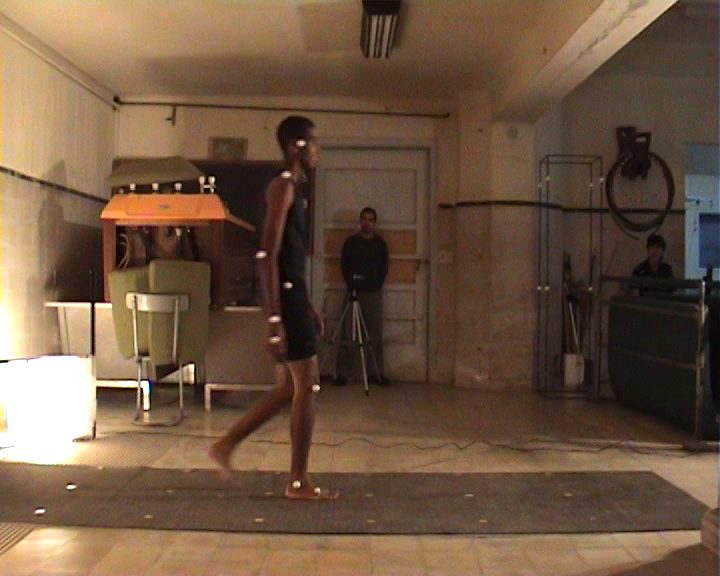
\includegraphics[scale=0.10]{imagenes/abel_original_video.png}\label{abelvideo}}\hspace{1 mm}
        {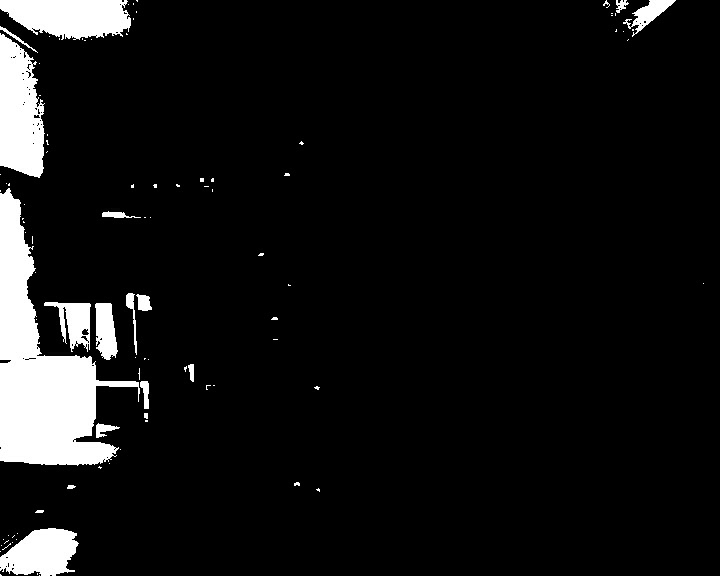
\includegraphics[scale=0.10]{imagenes/abel_original_filtro.png}\label{abelfiltro}}
        {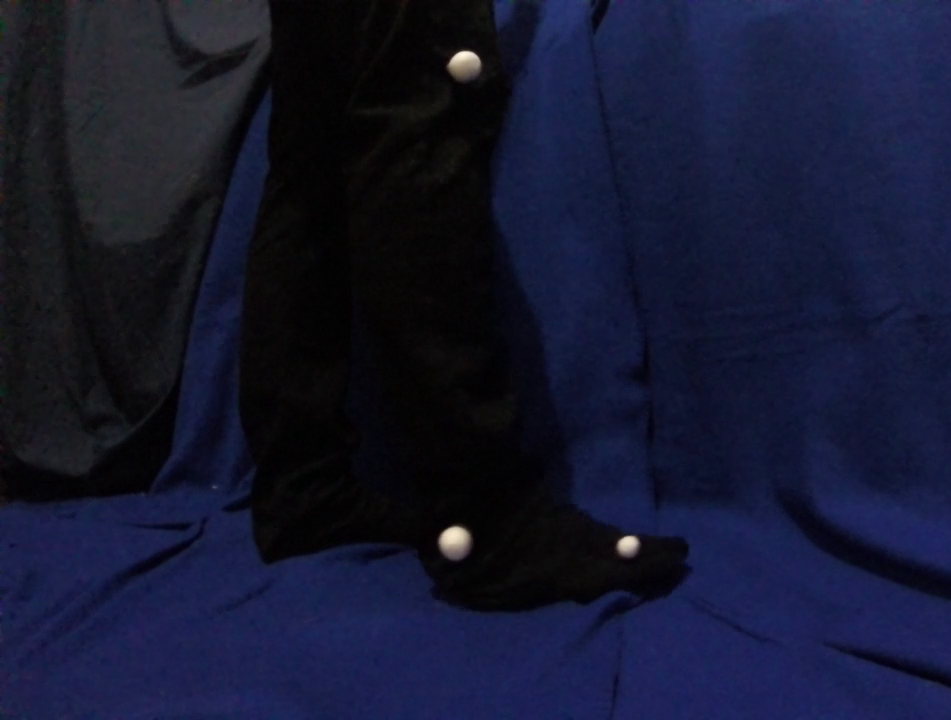
\includegraphics[scale=0.07]{imagenes/orig.png}\label{abelvideo2}}\hspace{1 mm}
       % {
\includegraphics[scale=0.07]{imagenes/filtr.png}\label{abelfiltro2}}\hspace{1 mm}
        {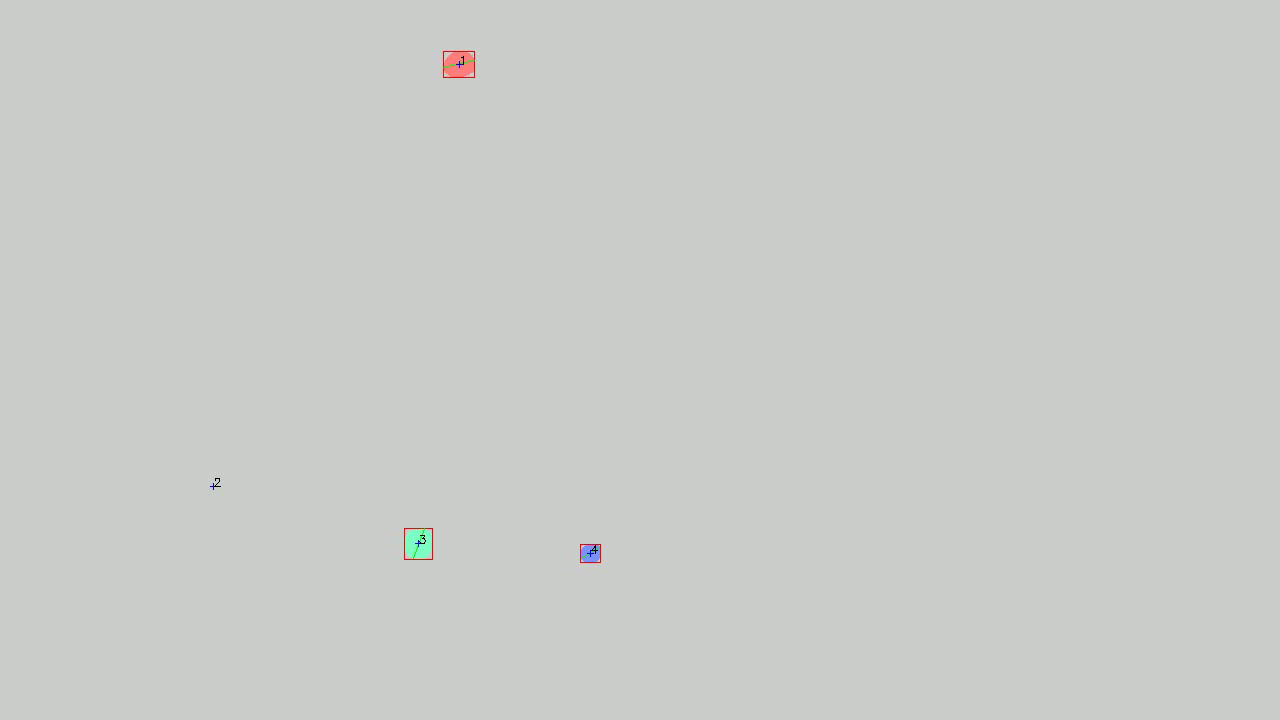
\includegraphics[scale=0.07]{imagenes/detect.png}
        \label{abeldetect}}
      \caption{%Entradas y salidas de cada etapa del bloque de deteción.
       %\textbf{(\ref{abelvideo})} 
       \textit{Left}: original image from a sequencue without capture hypothesis. 
       \textit{Left center}: segmentation results without capture hypothesis.
       % \textbf{(\ref{abelvideo2})} 
       \textit{Right center}: Original capture from a real sequence under capture hypothesis.
       % \textbf{(\ref{abelfiltro2})} Imagen filtrada con el umbral de Otsu. \textbf{(\ref{abeldetect})}
       \textit{Right}: Detected markers.}  
      \label{ejemploabelumbr2}
\end{figure}
%\vspace{-0.6cm}

\section{Discusión y análisis de resultados}


\section{Conclusiones}
%conclusiones, pendientes, etc

En esta sección se evaluarán las conclusiones obtenidas a partir de lo realizado en el proyecto. Las mismas se pueden separar en conclusiones generales, y en particulares de los capítulos vistos anteriormente.

Como conclusiones generales se presentan las siguientes:
\begin{itemize}
\item Se cumplió el objetivo principal: se logró obtener un sistema completo que a partir de las capturas de video de una persona en un ambiente de laboratorio con las condiciones adecuadas, obtiene la posición 3D de  los marcadores presentes en el cuerpo de dicha persona, logrando representar su movimiento con una presición del orden del centímetro.
\item Se logró relevar la literatura existente, y se realizó una clasificación de los documentos de acuerdo a la relevancia que prestan para construir un sistema de estas características. 
\item Se relevó el software existente, y se buscaron implementaciones en matlab, C/C++ y otros lenguajes, pero no se encontró un software Open Source que se adaptara a las características necesarias para utilizar de base en este proyecto. Debido a esto, se decidió implementar los bloques por cuenta propia, utilizando algunos algoritmos básicos de procesamiento de imagenes ya implementados o realizados especificamente para este proyecto. Esta etapa por momentos tuvo un carácter más de investigación científica que de proyecto ingenieril.
\item Se identificaron los distintos casos de uso, y se decidió implementar el sistema en base al caso de uso de marcha.
\item Se lograron implementar los 4 grupos de algoritmos principales que componen la aplicación: calibración, detección de marcadores, estimación de pose (o reconstrucción) y seguimiento.
\item Se generó un sistema que integra los 4 bloques nombrados en el punto anterior, y que dada la entrada definida obtiene la salida esperada.
\item Se elaboró una interfaz gráfica de usuario (GUI) básica para que el sistema pueda ser utilizado de una forma más práctica y amigable por el usuario.
\item Se buscaron bases de datos que se encuentren dentro de las hipótesis del problema, de forma tal de probar el mismo para diferentes casos y evaluar su rendiemiento. Debido a que no se encontró ninguna base de datos disponible que cumpla con las características deseadas, se elaboró una en base a secuencias sintéticas generadas en Blender.
\item Se generó un conjunto de benchmarks\footnote{Herramientas de evaluación de performance.}, capaces de obtener una buena medida del rendimiento del sistema. 
\end{itemize}

A continuación, se plantean las conclusiones específicas de las etapas principales del proyecto:
\begin{itemize}
	\item Relevamiento bibliográfico
	\begin{itemize}
		\item No se encontraron implementaciones de sistemas de captura de movimiento Open Source con las características del sistema de este proyecto. 
	\end{itemize}
	\item Base de datos
	\item Calibración
	\item Detección de marcadores
	\begin{itemize}
		\item Se logró implementar un conjunto de algoritmos capaces de detectar la posición 2D de los marcadores en el cuerpo del paciente para todo instante de tiempo y exponer los resultados en un archivo XML. 
		\item Los resultados correspondientes a las pruebas con secuencias cintéticas fueron muy buenos, logrando un error que en la mayoría de los casos se ubicó por debajo de los 4 píxeles.
		\item Por el lado del procesamiento de secuencias reales, no se consiguieron secuencias que estén exactamente en las hipótesis del probelma. Aún asi, se realizaron pruebas con secuencias que se asemejaban a las condiciones necesarias obteniendo buenos resultados al extraer el fondo de la captura.
		\item Se observó que para ambientes donde las condiciones se mantienen constantes a lo largo del tiempo (como por ejemplo en un laboratorio), el umbral no cambia significativamente su valor, pudiendose utilzar un valor constante en el para toda una secuencia. Esto permite ahorrar tiempo de procesamiento y reduce el costo computacional de la detección.
		\item Se observó que se puede mejorar la detección, ajustando los valores de las constantes $A$ y $B$ del filtro circular (ver seccióm \ref{implementSegment}) de forma tal de hacer el filtro más selectivo o menos.
	\end{itemize}
	\item Reconstrucción
	\item Segumiento
	\item Medida de performance
	\begin{itemize}
		\item Se obtuvo una precisión en la detección de los marcadores, del orden del centímetro.
		\item El máximo error no superó los 5 cm.
		\item Se obtuvieron muy buenos resultados, logrando reconstruir todos los marcadores en toda la secuencia hasta con un mínimo de 6 cámaras. Con menos cámaras se pierden marcadores ocasionalmente.
		\item Para el caso de 6 cámaras, la correcta detección del movimiento depende de la posición que tengan estas en el espacio.
	\end{itemize}
\end{itemize}

Cabe destacar que por temas de cronograma y de presupuesto, en muchos aspectos no se utilizó la tecnología más moderna (por ejemplo sensores infrarrojos, cámaras de mejor calidad, etc.) que de haberlas utilizado se hubiesen logrado mejores resultados. Si bien esta primera versión del sistema no está a la altura de los sistemas comerciales vistos en este documento, se logró dar el primer paso y se dejaron todas las condiciones necesarias para poder continuar con el proyecto y llevar el mismo al nivel de las otras herramientas.

Quedan como tareas pendientes para etapas futuras:
\begin{itemize}
	\item Probar el sistema en un laboratorio con las características definidas en este proyecto y con más de 6 cámaras previamente calibradas.
	\item Adaptar el sistema para otros casos de uso además de la marcha.
	\item Robustecer la segmentación, ya sea agregando algoritmos que complementen la umbralización de Otsu\cite{otsu} o cambiando la umbralización por un algoritmo más complejo.
	\item Mejorar la interfáz gráfica de usuario, haciéndola más amigable e intuitiva, de forma tal que el especialista pueda utilizarla como una aplicación de usuario.
	\item Realizar un manual de usuario.
\end{itemize}

\begin{thebibliography}{1}
\label{Referencias}

\bibitem{herda} Herda L., Fua P., Plankers R., Boulic R. Using skeleton-based tracking to increase the reliability of optical motion capture.Human movement science, 20(3), 313-341, 2001.
\bibitem{griegos} Malik N., Dracos T. \& Papantoniou D. (1993). Particle tracking in three-dimensional turbulent flows - Part II: Particle tracking, Experiments in Fluids, 15:279–294.
\bibitem{faugueras} Faugeras o., Robert L. What can two images tell us about a third one. International Journal of Computer vision, 18(1), 485-492,1996.
\bibitem{colombianos} C.A.Diaz, M.L.Toro, J.C.Forero, A.Torres Detección, rastreo y reconstrucción tridimensional de marcadores pasivos para análisis de movimiento humano. Cinemed iii
Revista ingeniería Biomédica issn 1909-9762, volumen 3, número 6, julio-diciembre 2009, págs. 56-67 Escuela de Ingeniería de Antioquia-Universidad ces, Medellín, Colombia
\bibitem{surveyThreshold} M.Sezgin,B.Sankur, “Survey over image thresholding techniques and quantitative performance evaluation”, Journal of Electronic Imaging 13(1), 146–165 (January 2004).
\bibitem{histImgRef} http://deploy.virtual$\-$labs.ac.in/labs/cse19/theory.php?exp=segment
\bibitem{Gonzalez} Digital Image Processing. Rafael Gonzalez  \& Richard Woods.
\bibitem{smooth} pág. 174, sección 3.5 Digital Image Processing. Rafael Gonzalez  \& Richard Woods.
\bibitem{tophat} pág. 692, sección 9.6.3 Digital Image Processing. Rafael Gonzalez  \& Richard Woods.
\bibitem{segment} pág. 760, sección 10.3 Digital Image Processing. Rafael Gonzalez  \& Richard Woods.
\bibitem{otsu} Nobuyuki Otsu (1979). "A threshold selection method from gray-level histograms". IEEE Trans. Sys., Man., Cyber.
\bibitem{implementacionOtsu} Matías Tailanian, Juan Cardelino. https://github.com/martin-etchart/kde 24/11/2014.
\bibitem{bayes} pág. 894, sección 12.2.2 Digital Image Processing. Rafael Gonzalez  \& Richard Woods.
\bibitem{procImg} D. Phillips; “Image Processing in C: Analyzing and Enhancing Digital Images”, RandD Publications, 1994
\bibitem{opencv} http://opencv.org/
\bibitem{cvblob} https://code.google.com/p/cvblob/
\bibitem{betweenvarianze} sección 4.4.4, http://homepages.inf.ed.ac.uk/rbf/CVonline/LOCAL{\_}COPIES/MORSE/threshold.pdf
\bibitem{kinect} http://www.xbox.com/es-ES/Kinect
\bibitem{xml} http://es.wikipedia.org/wiki/Extensible{\_}Markup{\_}Language
\bibitem{HSV} Shamik Sural, Gang Qian and Sakti Pramanik (2002). "Segmentation And Histogram Generation Using The HSV Color Space For Image Retrieval". Michigan State University, USA.
\bibitem{defBlob} http://en.wikipedia.org/wiki/Binary{\_}large{\_}object

\end{thebibliography}

\end{document}